\chapter{Values}

\begin{quote}
"Who looks outside, dreams; who looks inside awakens." Jung 
\end{quote}
\newpage

\begin{figure}[!h]
\begin{center}
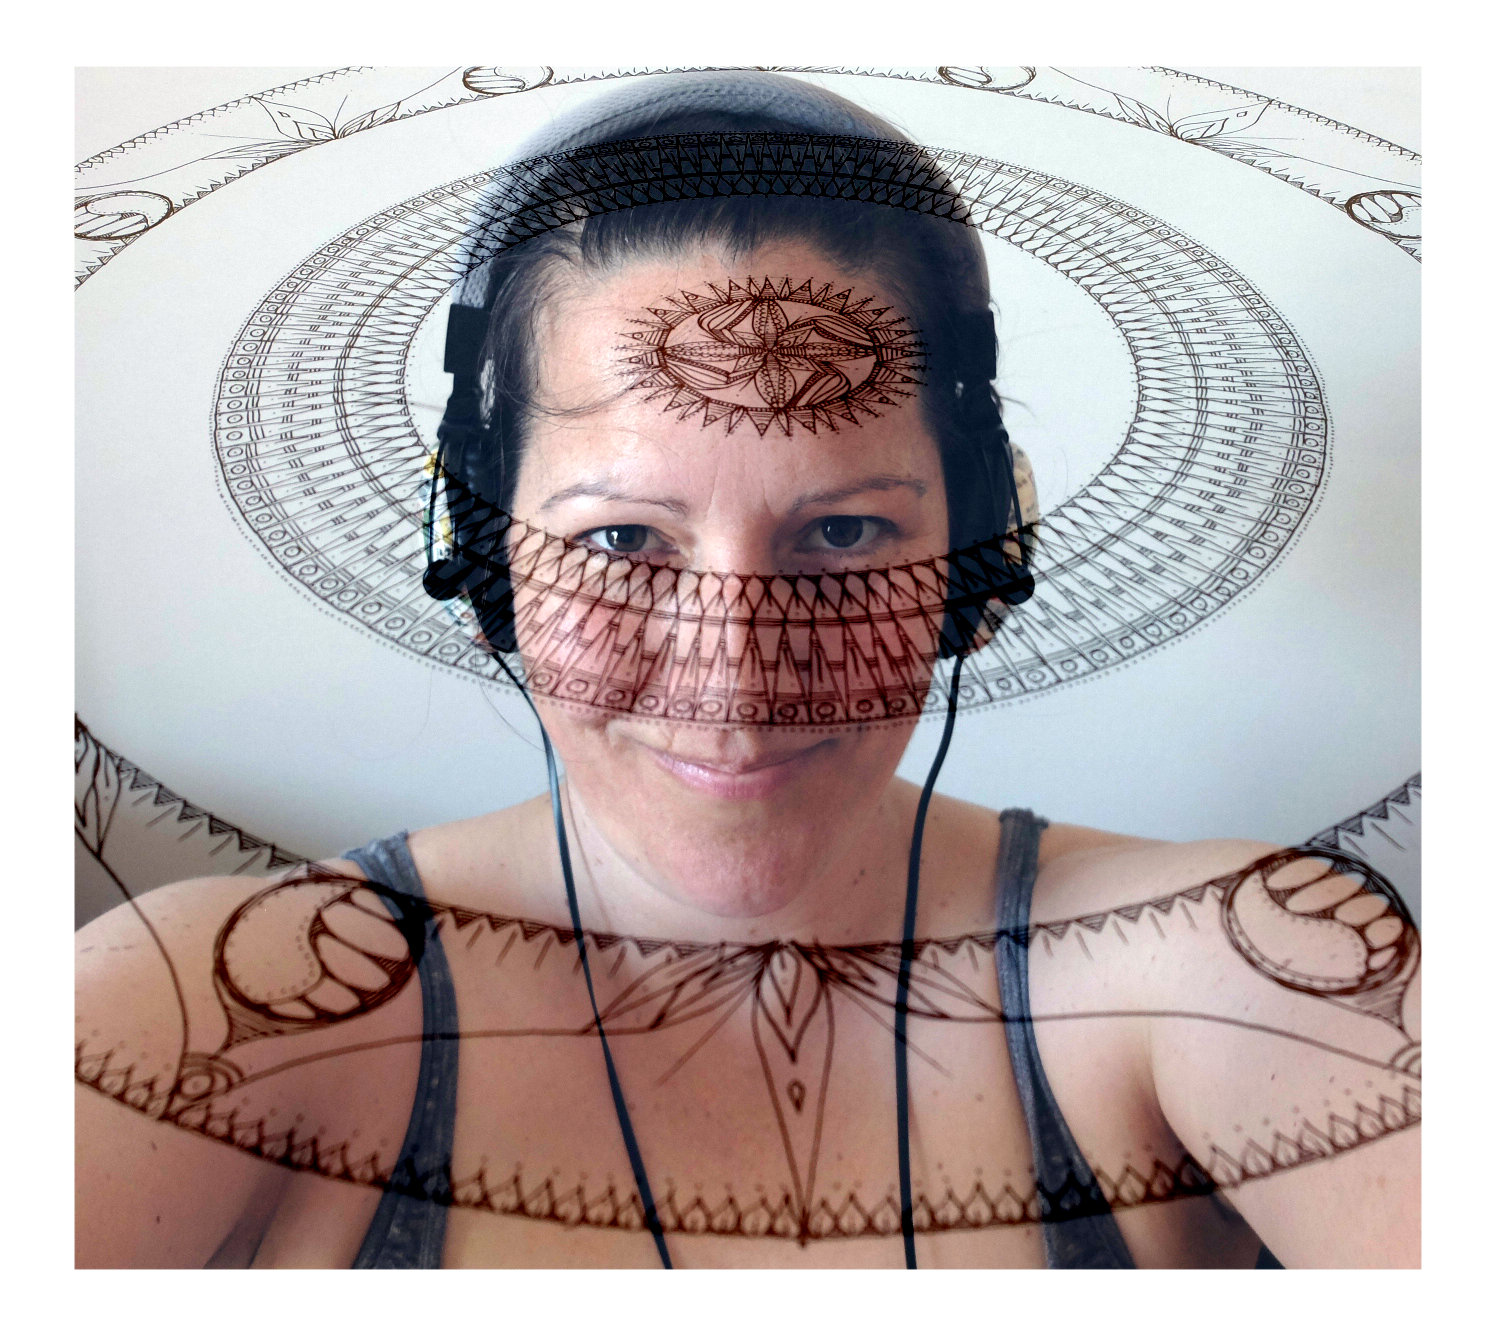
\includegraphics[scale=.3]{../eps/My_values.eps} 
\caption{My values}
\label{label}
\end{center}
\end{figure}

%FIGURE 1-MY VALUES 

Values

I have come to a better understanding of my values and needs and have become wiser for it, through creating my conversations within the mandalas. It has been great to be able to witness my own emotional evolution. I feel that I have healed parts of myself that needed attention. I feel I have immersed myself within the mandalas in combination with other processes. My values and needs were submerged before starting my inquiry. 

My titles are formed when I look at the mandala and rely on my felt sense, as well as any imaginative visualisations that might spring to mind. It is very much a free writing exercise with my visual imagery which comes to the fore.

\begin{figure}[!h]
\begin{center}
\includegraphics[scale=.12]{../eps/Double_exposure_of_my_values.eps} 
\caption{Double exposure of my values }
\label{label}
\end{center}
\end{figure}

%FIGURE 2- DOUBLE EXPOSURE OF MY VALUES
\newpage
\section{Connection}

\begin{figure}[!h]
\begin{center}
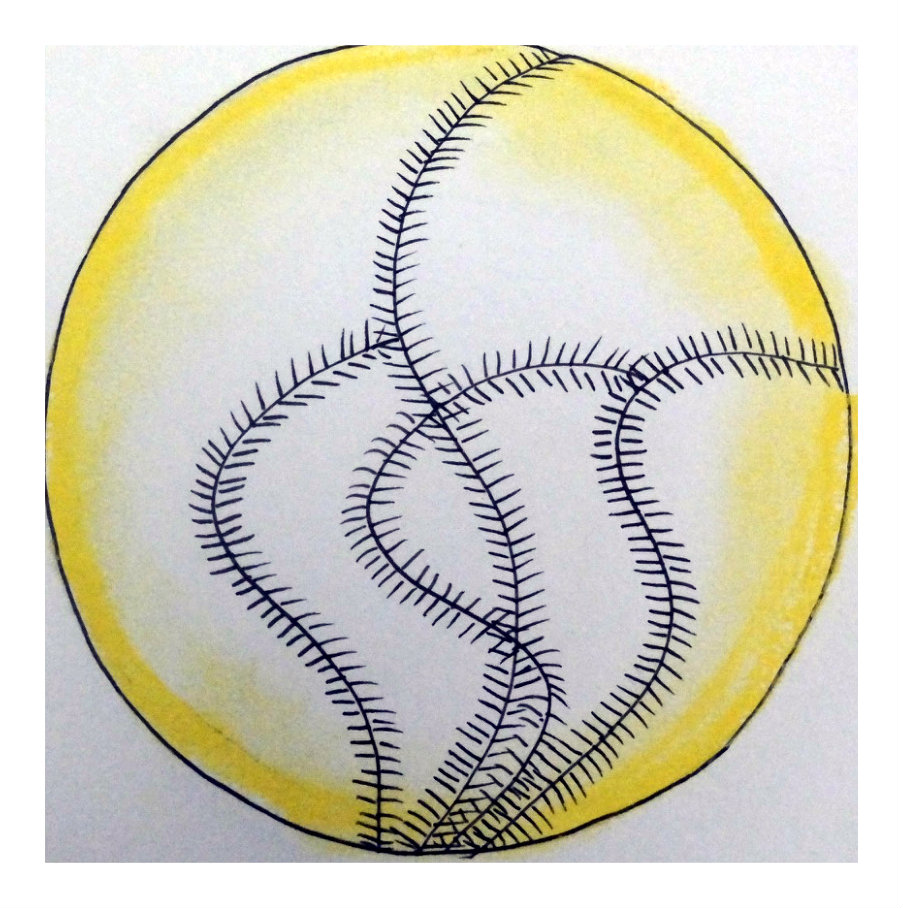
\includegraphics[scale=.2]{../eps/Connection-valueA.eps} 
\caption{Overlap, touch and sway in the wind}
\label{connection}
\end{center}
\end{figure}

%FIGURE 3-CONNECTION

The first value I have in my work and life is connection. It is nice to be awakened and realise that we live in a world where we are relational beings and connecting is an innate trait. As Buddha states 
\begin{quote} "All things appear and disappear because of the concurrence of causes and conditions. Nothing ever exists entirely alone; everything is in relation to everything else." 
\end{quote}

\newpage
\section{Clarity} 

\begin{figure}[!h]
\begin{center}
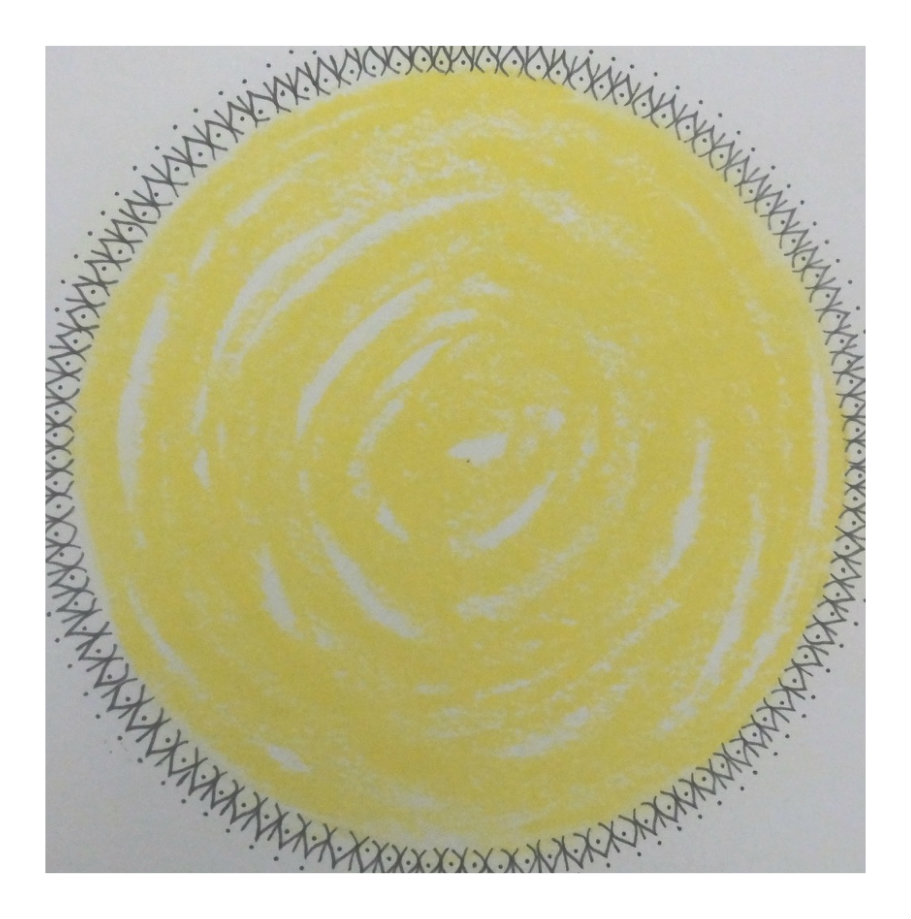
\includegraphics[scale=.2]{../eps/clarity.eps} 
\caption{Being able to understand peacefully}
\label{Clarity}
\end{center}
\end{figure}

%FIGURE 4-CLARITY

\begin{quote}
"If you want to understand the jungle, you cannot be content just to sail back and forth near the shore. Your'e got to get into it, no matter how strange or frightening it may seem."
\end{quote}

I value clarity, which is the quality of being able to easily see, hear and understand and to be able to understand not only the meaning within my experiences but the journey I took to arrive at these meanings. My thesis takes you through my process of finding clarity for myself and also describes why I value drawing mandalas from a therapeutic point of view. 

\newpage
\section {Imaginative visualisations}

\begin{figure}[!h]
\begin{center}
\includegraphics[scale=.2]{../eps/imaginative_visualizations_.eps} 
\caption{ So much to learn, open and see}
\label{Imaginative visualisations}
\end{center}
\end{figure}

%FIGURE 5-IMAGINATIVE VISUALISATIONS

My third value is about the power of imaginative visualisations. Elkins states that \begin{quote}
"The conscious mind engages in a more logical thought and rational thinking. The unconscious mind processes information in a more experiential manner and responds to feelings, images and suggestions more automatically" (pp59 Gary Elkins, )date.)
\end{quote}



Hypnotic relations therapy principles and applications) Hence, if we are aware that there is so much beneath the surface which is not conscious, and allow ourselves to be open to our imaginations, we may bring into awareness the little gems that have been outside our consciousness through this experiential explorations. Thus, I agree with McNiffs comment when he states: 

\begin{quote}
"I prefer a more imaginative attitude that views the image as a step a head of the reflecting mind, as a guide who shows me where I can go and what I can be." (McNiff, p 67,2004)(Art Heals) 
\end{quote}

\newpage
\section{Emergence}


\begin{figure}[!h]
\begin{center}
\includegraphics[scale=.1]{../eps/Emergence_A.eps} 
\caption{Openness to let things naturally form }
\label{Emergence}
\end{center}
\end{figure}

%FIGURE 6-EMERGENCE

My fourth value is emergence. To be able to let go and trust the process of emergence which in short is an intuitive improvisational quality and seems to derived from a felt resonance to the current moment.(Lett,p, 11, 2011)(making sense of our lives) As Merleau-Ponty states: 
\begin{quote}
"Thinking a movement is destroying the movement." (Merleau-Ponty 1962)
\end{quote}
 and so when we let our reflexive-reflective interactions flow into awareness we reap the benefits.






